\documentclass{article}
\usepackage[utf8]{inputenc}
\usepackage{amssymb, amsmath,hyperref,verbatim,listings,graphicx,subfigure,fullpage}

\begin{document}

\title{UML computer project 1}
\author{
Juha-Antti Isojärvi\\
013455341 \\
Department of Mathematics and Statistics\\
Master student
\and
Mikko Sysikaski\\
013573016\\
Department of Computer Science\\
Master student}
\date{}
\maketitle

\section{Exercise set 1}
\subsection{Exercise 1}
First we were given a plot of twodimensional data, and were asked to
create similar data artificially. The distribution of the data looked
similar to the twodimensional gaussian or multinormal
distributions. Therefore we decided to generate points from a
gaussian distribution. 

A random vector $X = (X_1, X_2, \dots, X_n)$ is standard normally
distributed, denoted $X \sim N_n(0,I)$, if its components $X_i$ are independent and normally
distributed with zero mean and unit variance. It is true, that the
mean vector $E(X) = 0$ and covariance matrix $Cov(X) = I_n$.

Now if a random vector 
\[
X = AU + \mu
\] 
is defined for some $U \sim N_n(0,I)$, and fixed $A \in \mathbb{R}^{m \times n}$
and $\mu \in \mathbb{R}^n$, then it is true that $E(X) = \mu$ and
$Cov(X) = AA^T$.

A random vector $X$ is multinormally
distributed, if it has the same
distribution as the random vector
\[
X = AU + \mu.
\]
Then it has mean $E(X) = \mu$ and covariance $Cov(X) = AA^T$. Denote
$Cov(X) \dot{=} \Sigma$. The multinormal distribution is denoted $X
\sim N_n(\mu,\Sigma)$.

It also holds, that if $X \sim N_n(\mu,\Sigma)$, and $B \in
\mathbb{R}^{m \times n}$ and $b \in \mathbb{R}^m$ are fixed, then 
\[
BX + b \sim N_m(B\mu + b, B \Sigma B^T).
\]

Now, one way of simulating gaussian twodimensional data, is to first
simulate twodimensional standard normally distributed, i.e. white, data, and then
affinely transform this data by multiplying with some matrix $A \in
\mathbb{R}^{2\times 2}$. The affinely transformed data has then a
gaussian distribution with zero mean and covariance $AA^T$.

So, we generated two random samples from a normal distribution and put these
together to form twodimensional white data. If one would plot this
data, one would see a spherical point cloud centered at zero. Then we
dilated this cloud in the $y$- and $x$-axis direction with multiplying by a dilation matrix $D$ and then rotated
the dilated data cloud with multiplying by a rotation matrix
$R_\theta$. The result was a sample from the 
distribution $N_2(0,AA^T)$, where $A \dot{=} R_\theta D$.

The resulting data cloud is centered at zero, and has elliptical
shape. The main axis of this data cloud has angle $\theta$ measured
form the $x$-axis. Our resulting four generated artificial data can be
seen plotted in Figure~\ref{fig:scatter}. 

This was a simple method for generating artificial twodimensional
gaussian data, with easy control of the direction and elongation of
the data cloud. Of course there are other methods as well. In the
$MASS$-package of $R$ there is a function mvrnorm, which takes as
inputs the mean vector and the covariance matrix and generates
gaussian data. The method implemented is the so called
Stetson-Harrison method, and we think it may be just what we used. We
didn't feel the need to get further into the details of this
method. Manipulation of the direction and the elongation of the data
cloud is always achieved by manipulation of the covariance matrix, as
in the method we described.

Another way of manipulating the direction and elongation of the data
cloud is by 'inverse' eigenvalue decomposition of the covariance
matrix. About this method more in section \ref{sec:subsection4}.
\subsection{Exercise 2}
The principal components of the first and the third point set are shown in Figure~\ref{fig:pcadir}.
\subsection{Exercise 3}
The Figure~\ref{fig:histo} contains the histograms obtained by projecting the points of the first point set on its principal components.
\subsection{Exercise 4}\label{sec:subsection4}
\subsection{Exercise 5}

\newcommand{\sscale}{0.5}
\begin{figure}\centering
	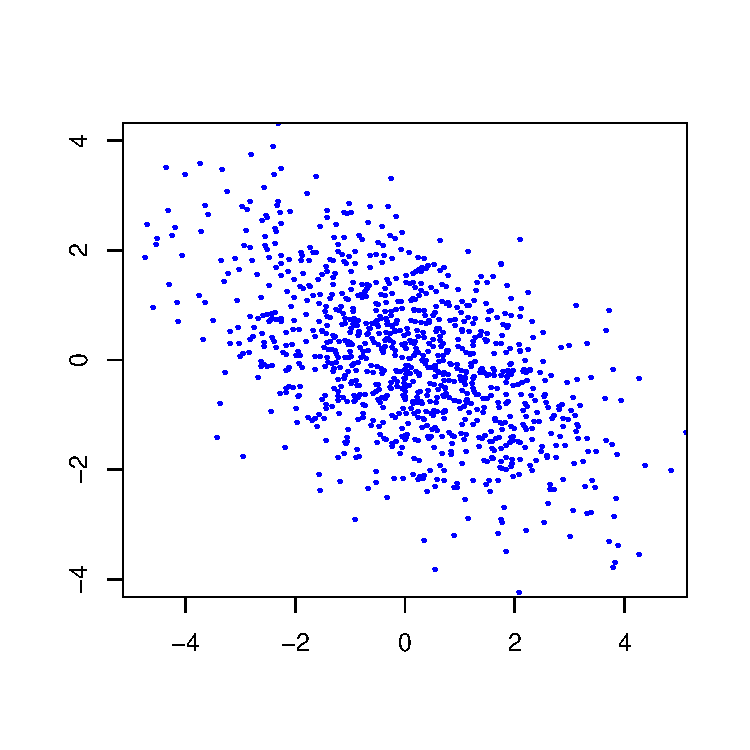
\includegraphics[scale=\sscale]{scatter1}
	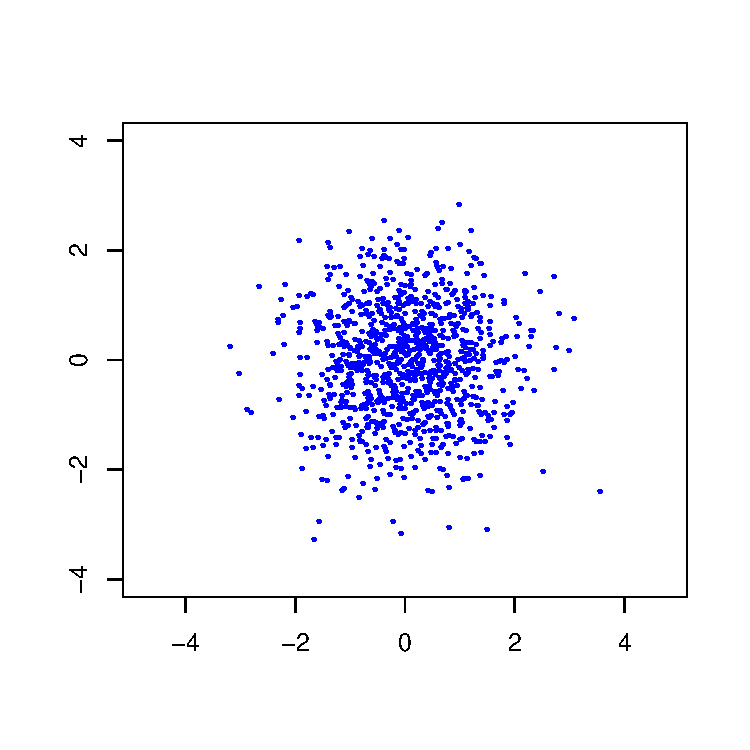
\includegraphics[scale=\sscale]{scatter2}

	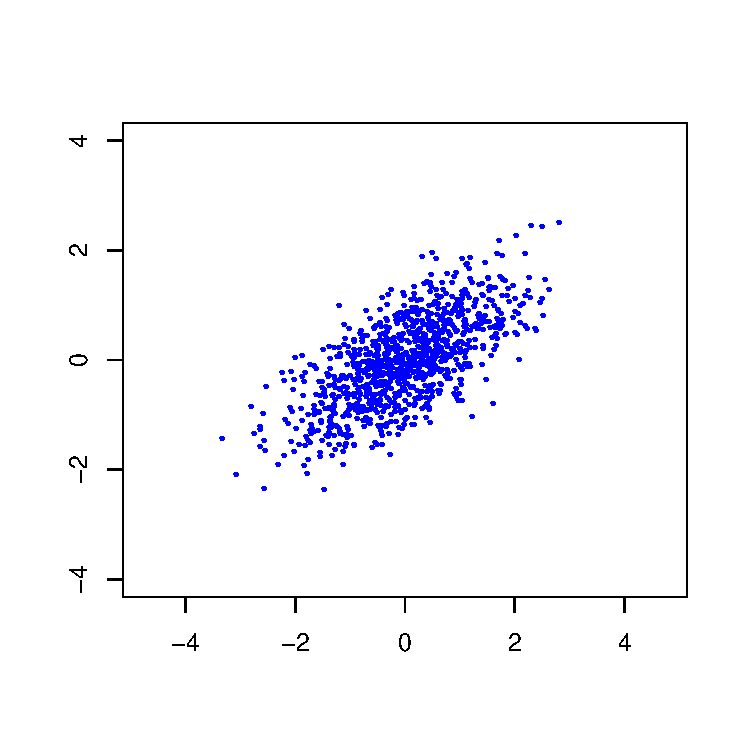
\includegraphics[scale=\sscale]{scatter3}
	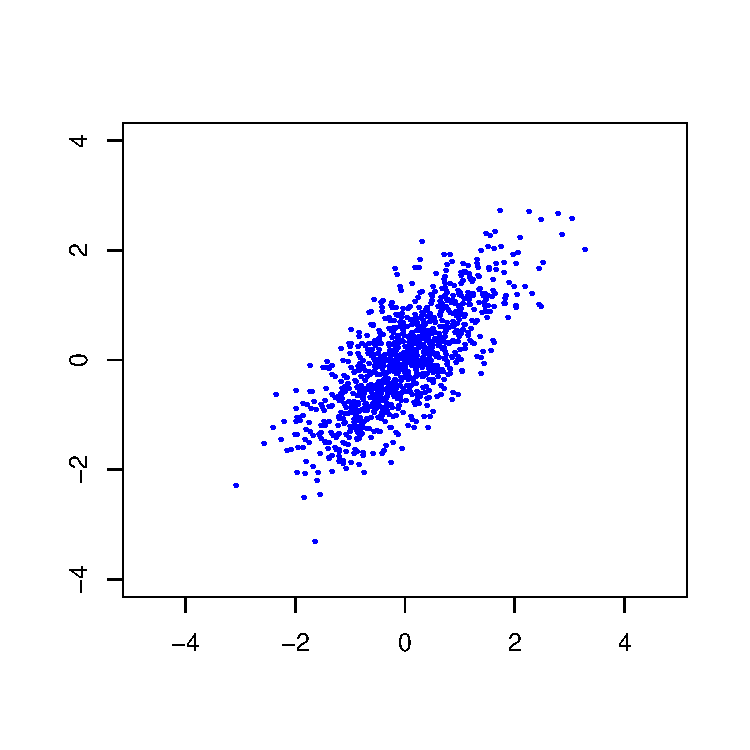
\includegraphics[scale=\sscale]{scatter4}
	\caption{The scatter plots of the data generated in task 1.1.} \label{fig:scatter}
\end{figure}
\begin{figure} \centering
	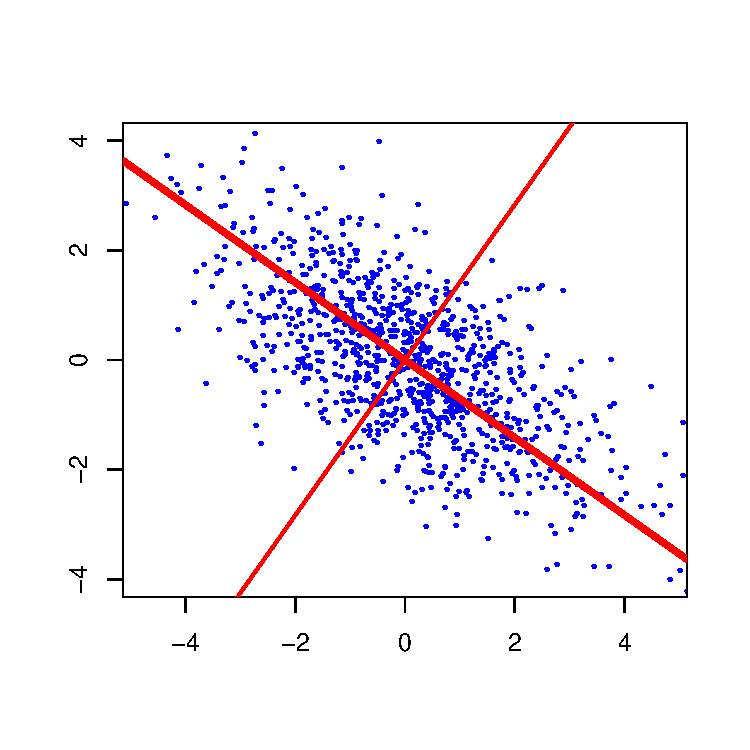
\includegraphics[scale=\sscale]{pcadir1}
	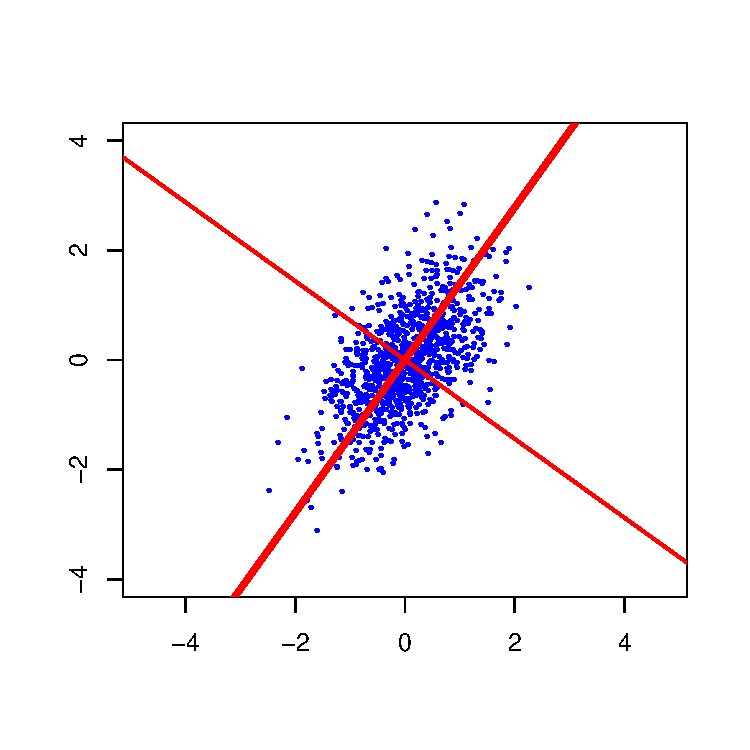
\includegraphics[scale=\sscale]{pcadir3}
	\caption{Principal components of the first and the third point set. The first PC is the bolder line.} \label{fig:pcadir}
\end{figure}
\begin{figure} \centering
	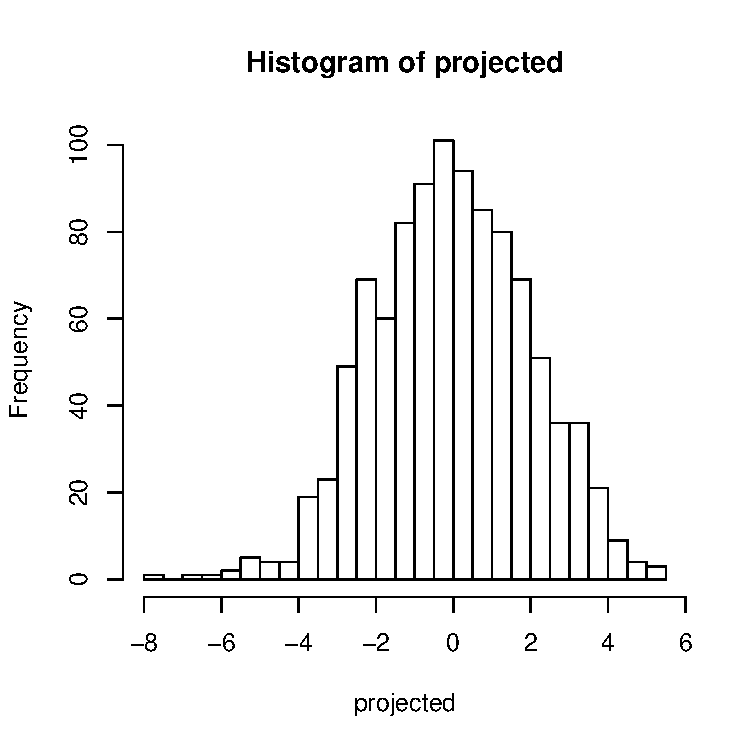
\includegraphics[scale=\sscale]{histo1-1}
	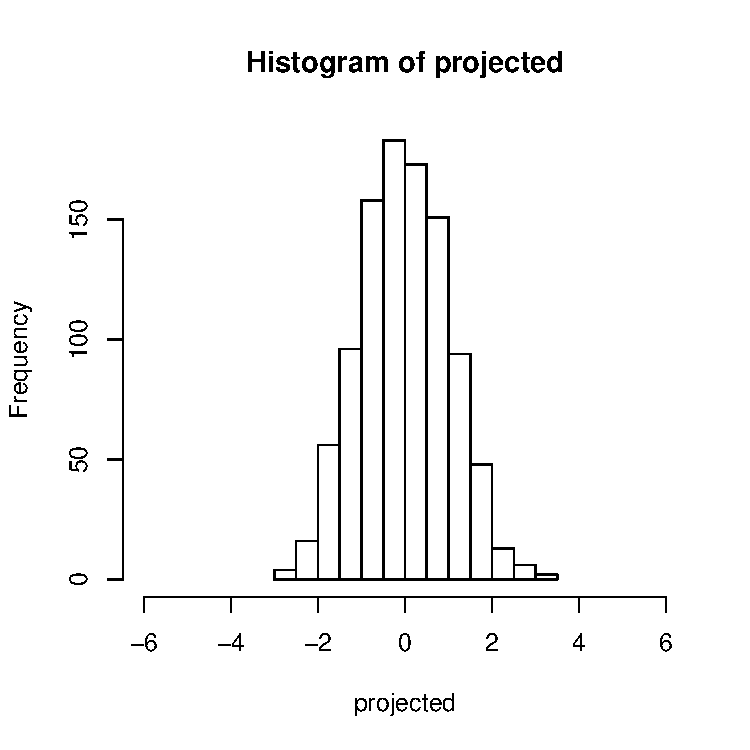
\includegraphics[scale=\sscale]{histo1-2}
	\caption{Histograms of the 1-dimensional data obtained by projecting the points of the first point set on its principal components.} \label{fig:histo}
\end{figure}
\begin{figure} \centering
	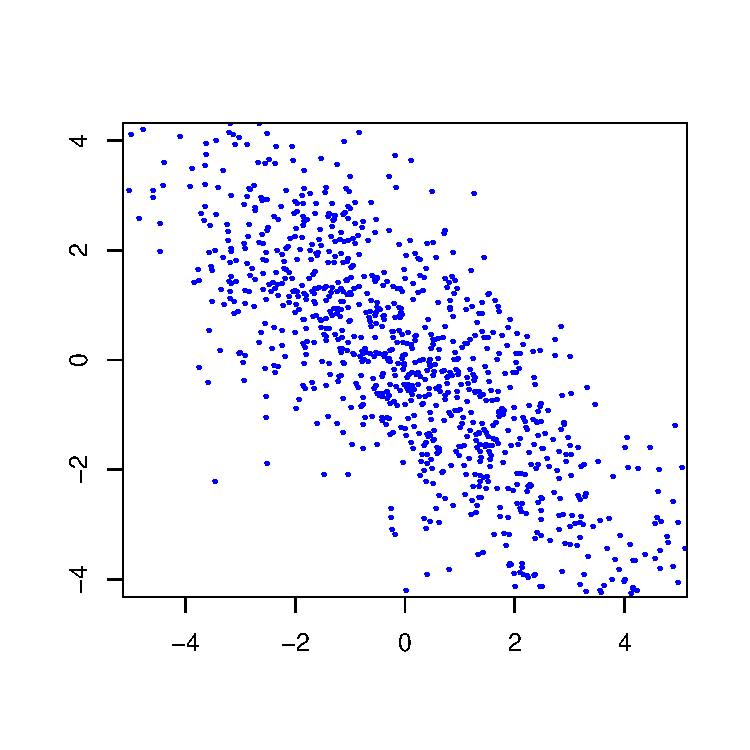
\includegraphics[scale=\sscale]{vscatter}
	\caption{} \label{fig:vscatter}
\end{figure}
\begin{figure} \centering
	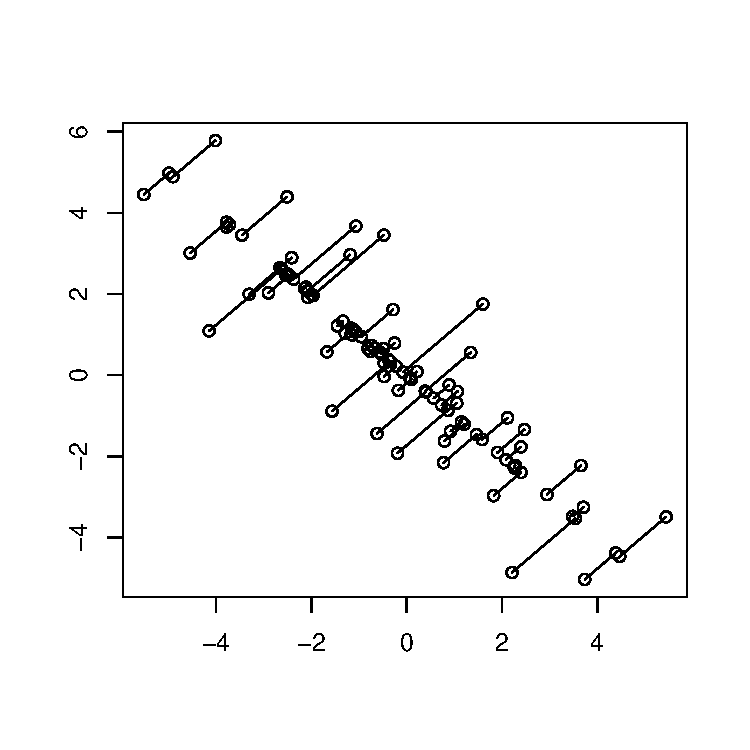
\includegraphics[scale=\sscale]{proj}
	\caption{} \label{fig:proj}
\end{figure}

\section{Exercise 2}
\newcommand{\X}{\ensuremath{\mathbf{X}}}
\subsection{}
The task was to do primary component analysis on the matrix
$$ X =
\begin{pmatrix}
	5 & 3 & 0 & 1 & -1 & -3 & 5 & 0 & -4 & -4 \\
	-2 & -1 & 0 & 0 & 1 & 4 & -3 & 1 & 5 & 3 \\
	0 & 1 & 4 & -1 & 0 & 5 & 5 & -5 & -3 & -3 \\
	0 & 2 & 3 & 0 & -1 & 3 & 3 & -7 & -2 & 0 \\
	3 & 4 & -2 & 1 & 3 & -3 & -3 & 2 & 0 & 0
\end{pmatrix}.
$$

The Figure~\ref{fig:42} displays the data and the original variables projected to the first two principal components.
\subsection{}
The amount of variance explained as a function of the number of principal components used is displayed in Figure~\ref{fig:varamount}. It can be seen that the projection to the first two components in Figure~\ref{fig:42} convey about 90.6\% of the information of the data.
\subsection{}
\subsection{}
The quartimax applied to the first two principal components of \X. Figure~\ref{fig:qmax} shows the projections of the variables on the rotated components. Note that the figure is the same as Figure~\ref{fig:42}, only rotated. The rotation doesn't change the subspace spanned by the principal components, so they explain the same amount of variance before and after rotation.

\begin{figure}\centering
	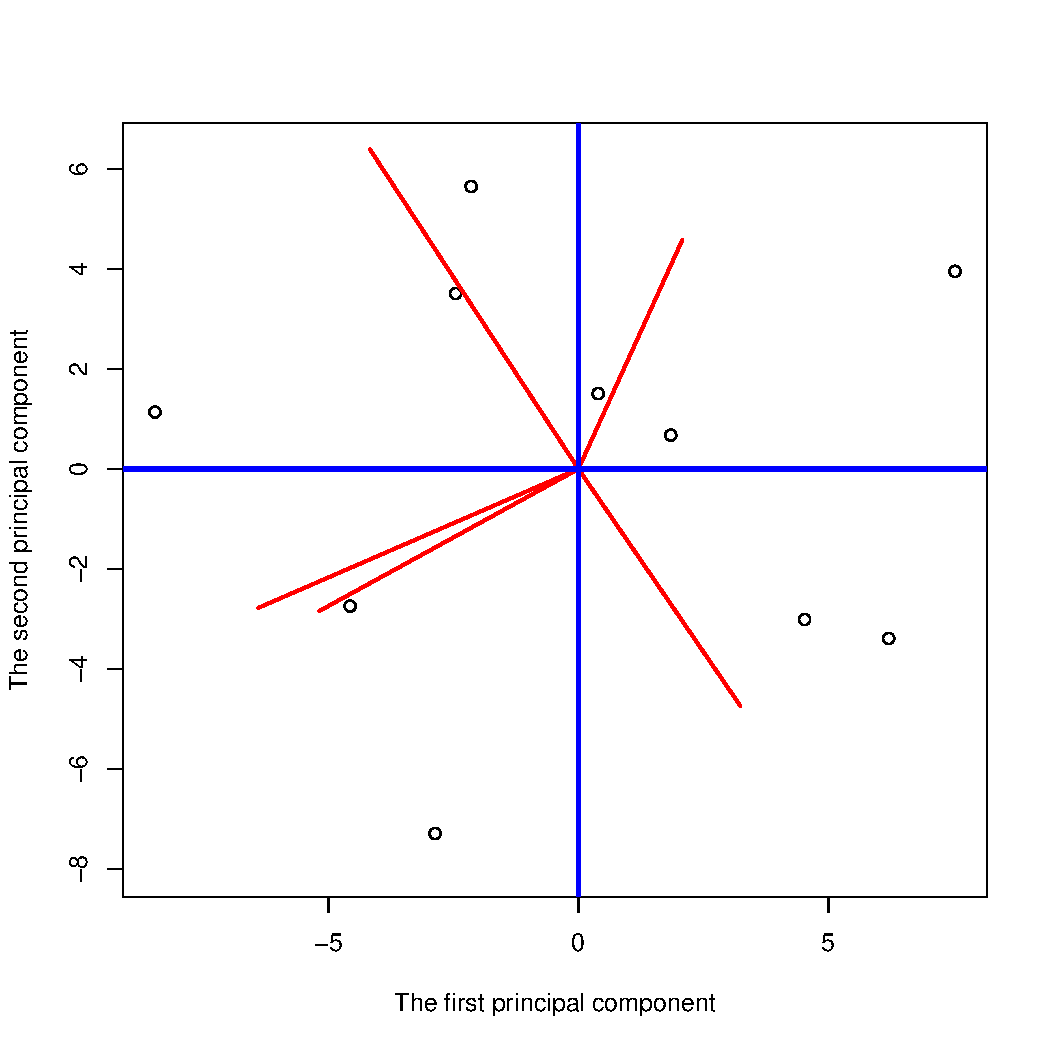
\includegraphics[scale=\sscale]{fig42}
	\caption{Reproduction of Figure~4.2 on the lecture notes. The blue points are the data points projected to the first two principal components. The red lines are the projections of the original coordinate axes.}\label{fig:42}
\end{figure}
\begin{figure}\centering
	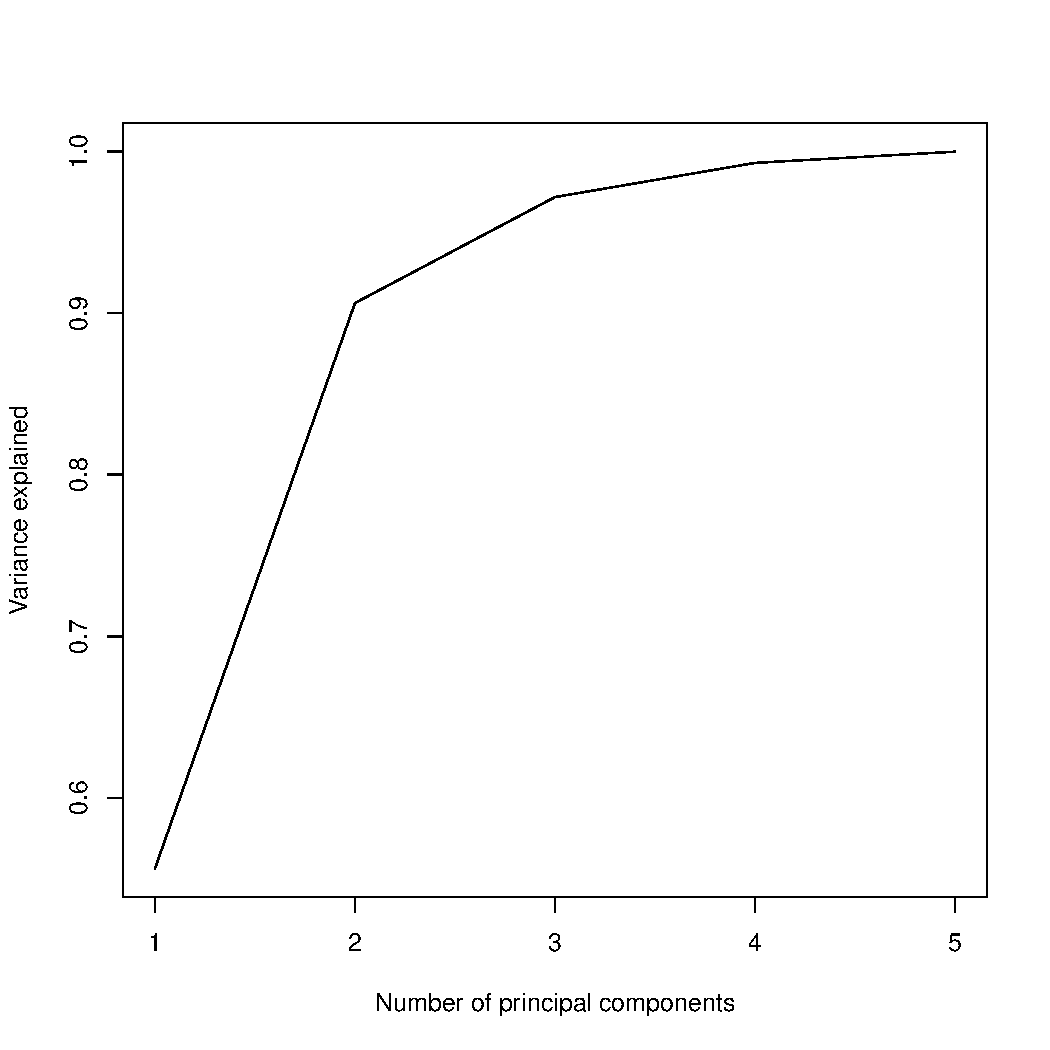
\includegraphics[scale=\sscale]{varamount}
	\caption{The proprotion of the variance explained by using only some of the principal components.}\label{fig:varamount}
\end{figure}
\begin{figure}\centering
	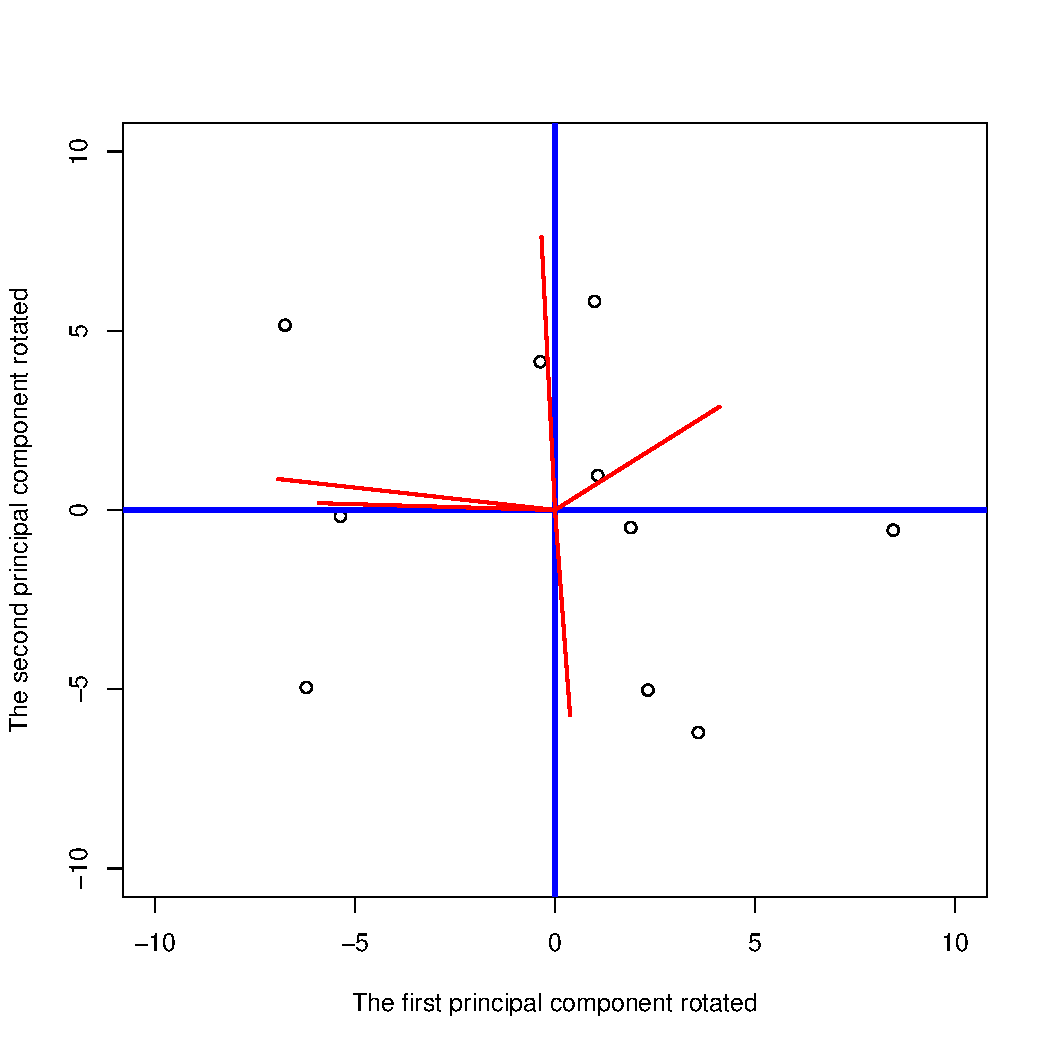
\includegraphics[scale=\sscale]{qmax}
	\caption{The projection to principal components after rotating them using the quartimax algorithm to have the original variables as close to the new coordinate axes as possible.}\label{fig:qmax}
\end{figure}

\section{Exercise 3}
\subsection{}
\subsection{}
\subsection{}
\subsection{}

\begin{figure}\centering
	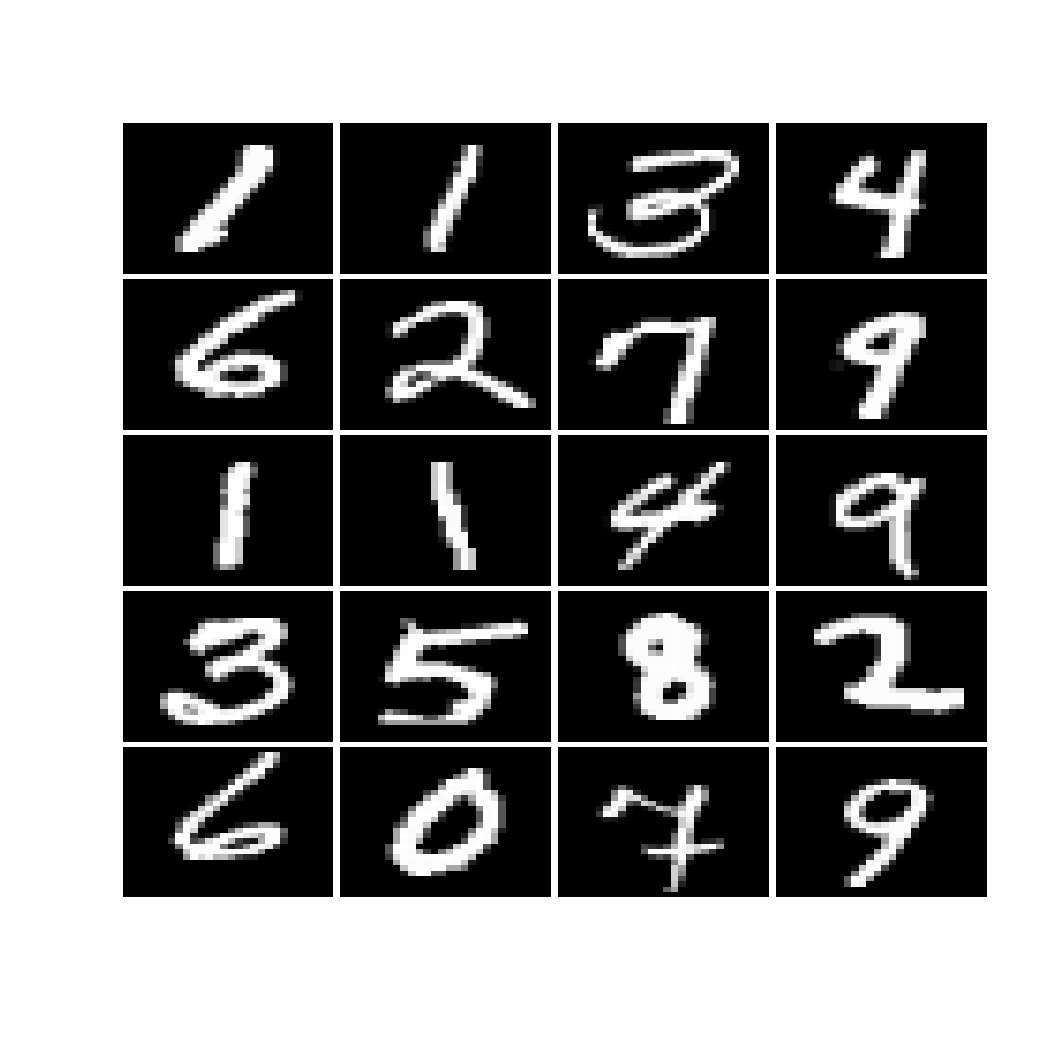
\includegraphics[scale=0.4]{digits}
	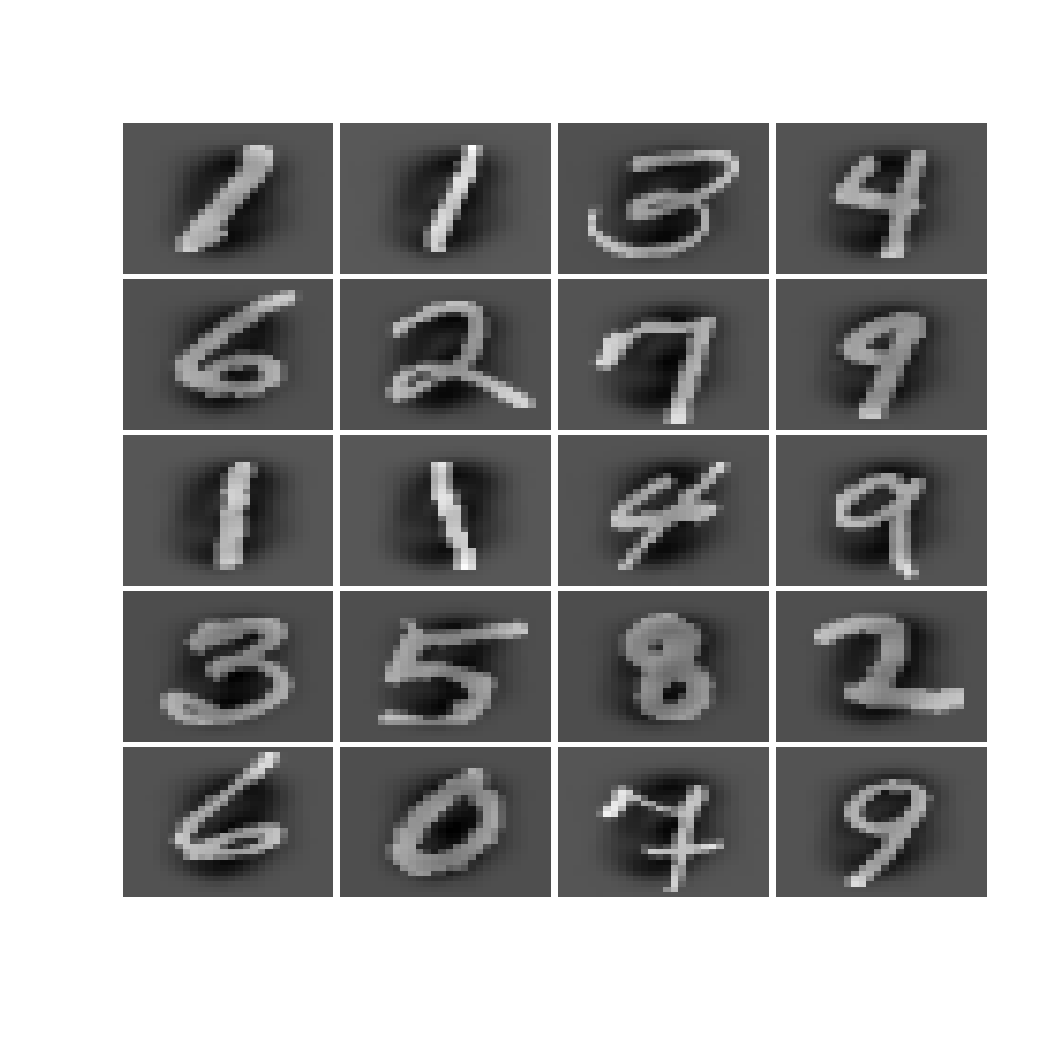
\includegraphics[scale=0.4]{digitspre}
	\caption{}\label{fig:digits}
\end{figure}
\begin{figure}\centering
	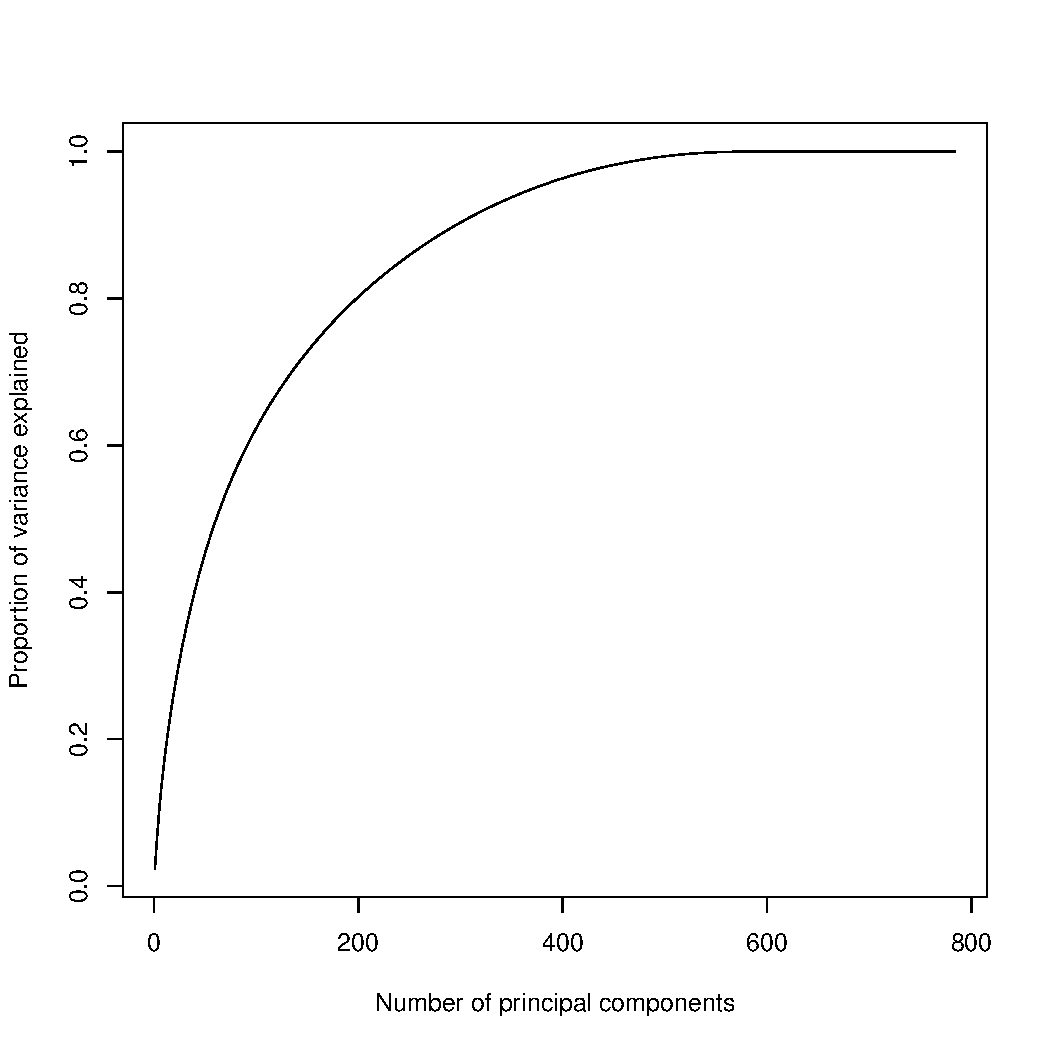
\includegraphics[scale=0.4]{pcavar}
	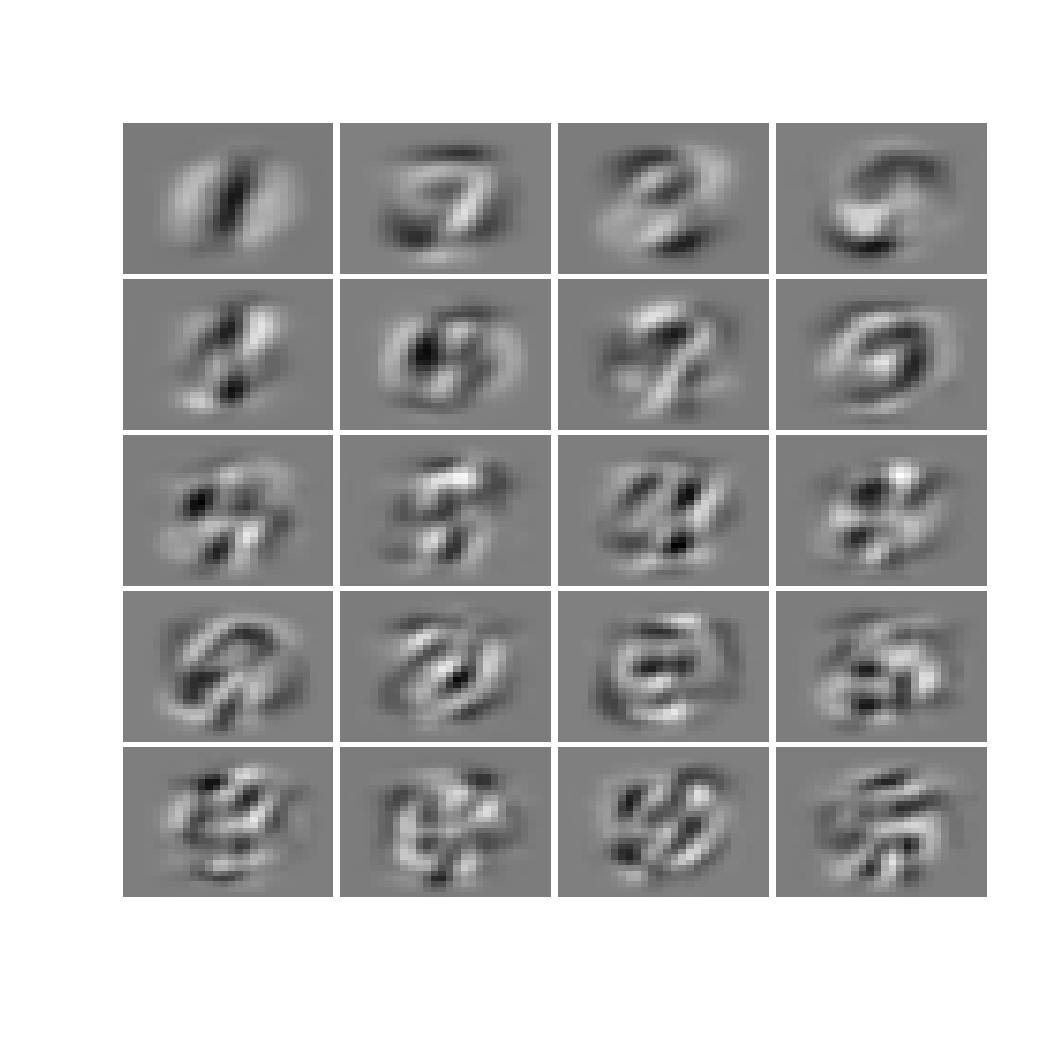
\includegraphics[scale=0.4]{pcanums}
	\caption{}\label{fig:pcavar}
\end{figure}
\begin{figure}\centering
	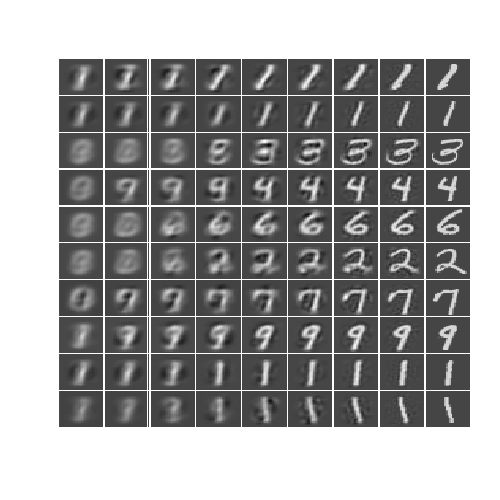
\includegraphics[scale=\sscale]{digitreduce}
	\caption{}\label{fig:reduce}
\end{figure}
\begin{figure}\centering
\newcommand{\dns}{0.4}
	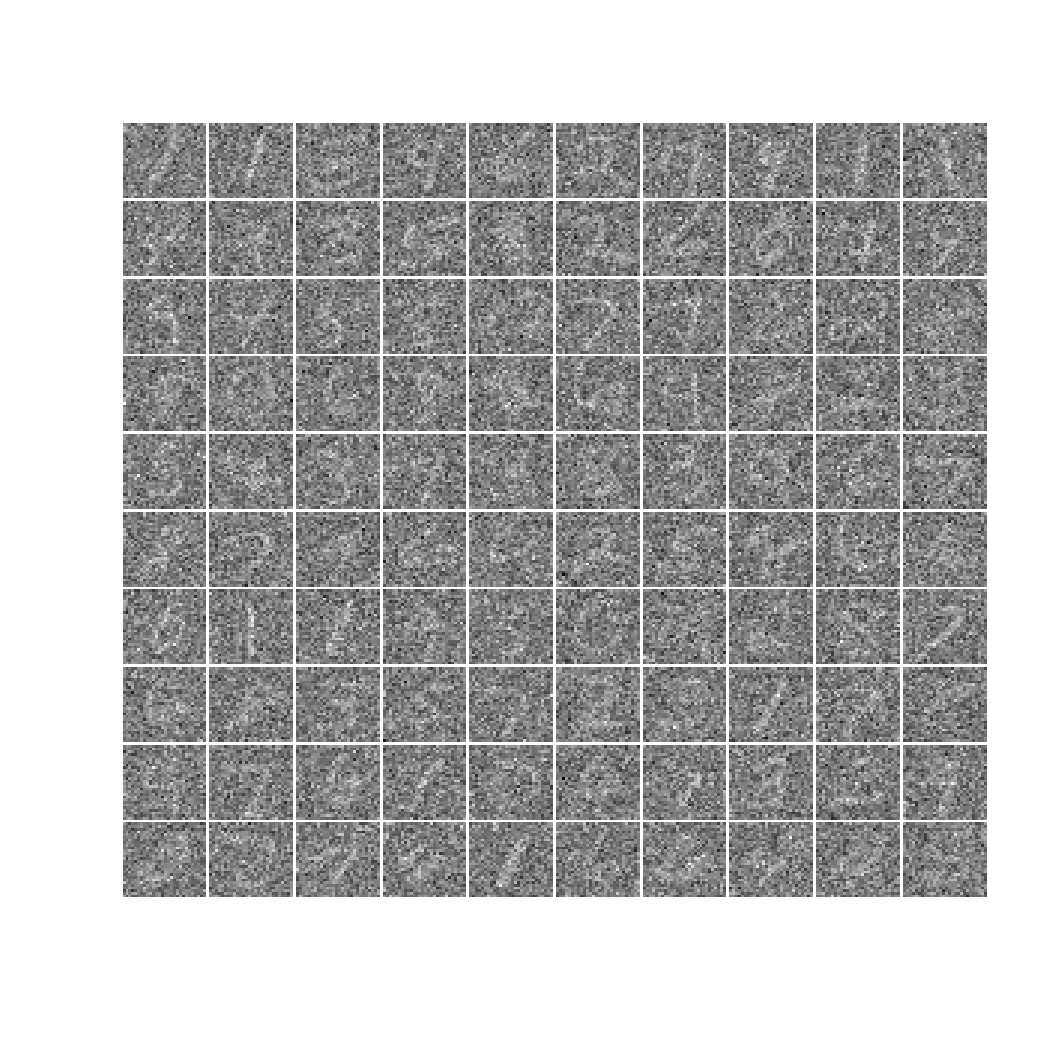
\includegraphics[scale=\dns]{noisy}
	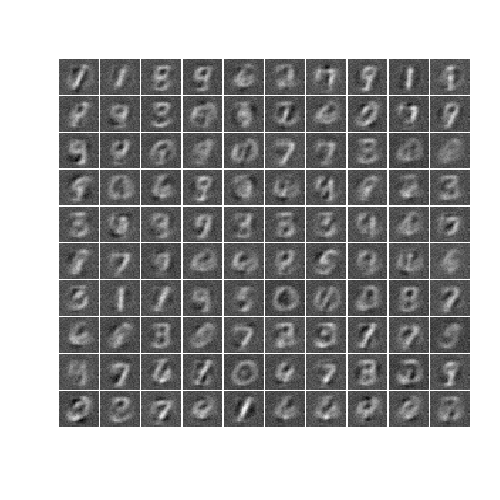
\includegraphics[scale=\dns]{denoise8}
	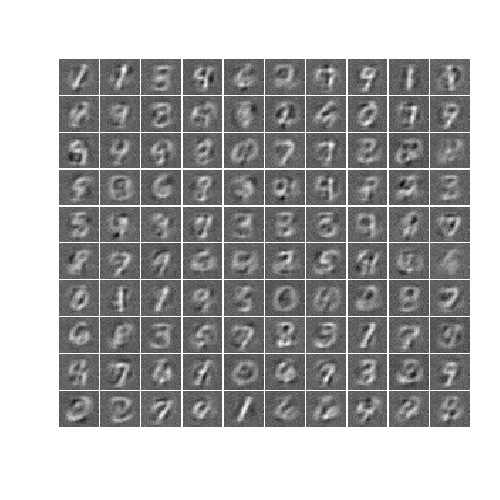
\includegraphics[scale=\dns]{denoise16}
	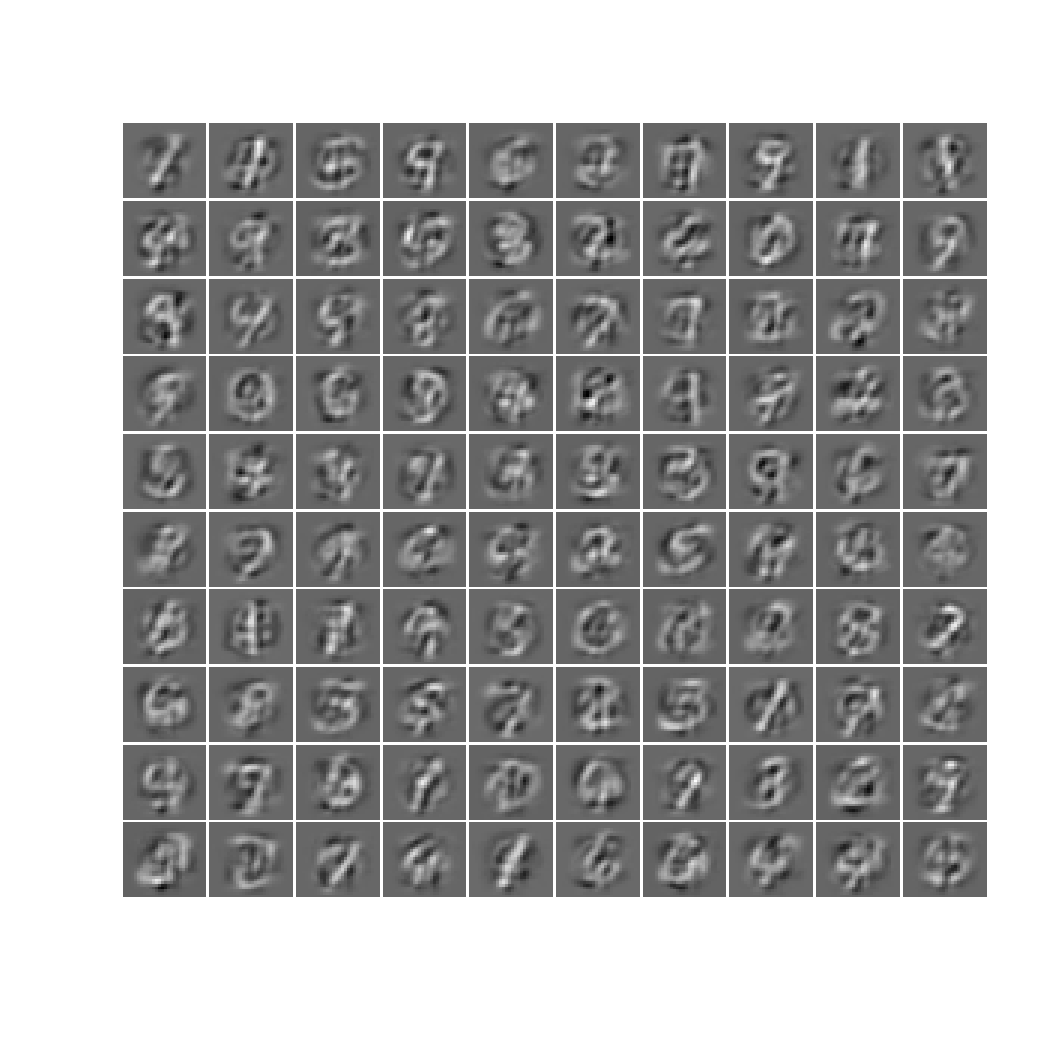
\includegraphics[scale=\dns]{denoise32}
%	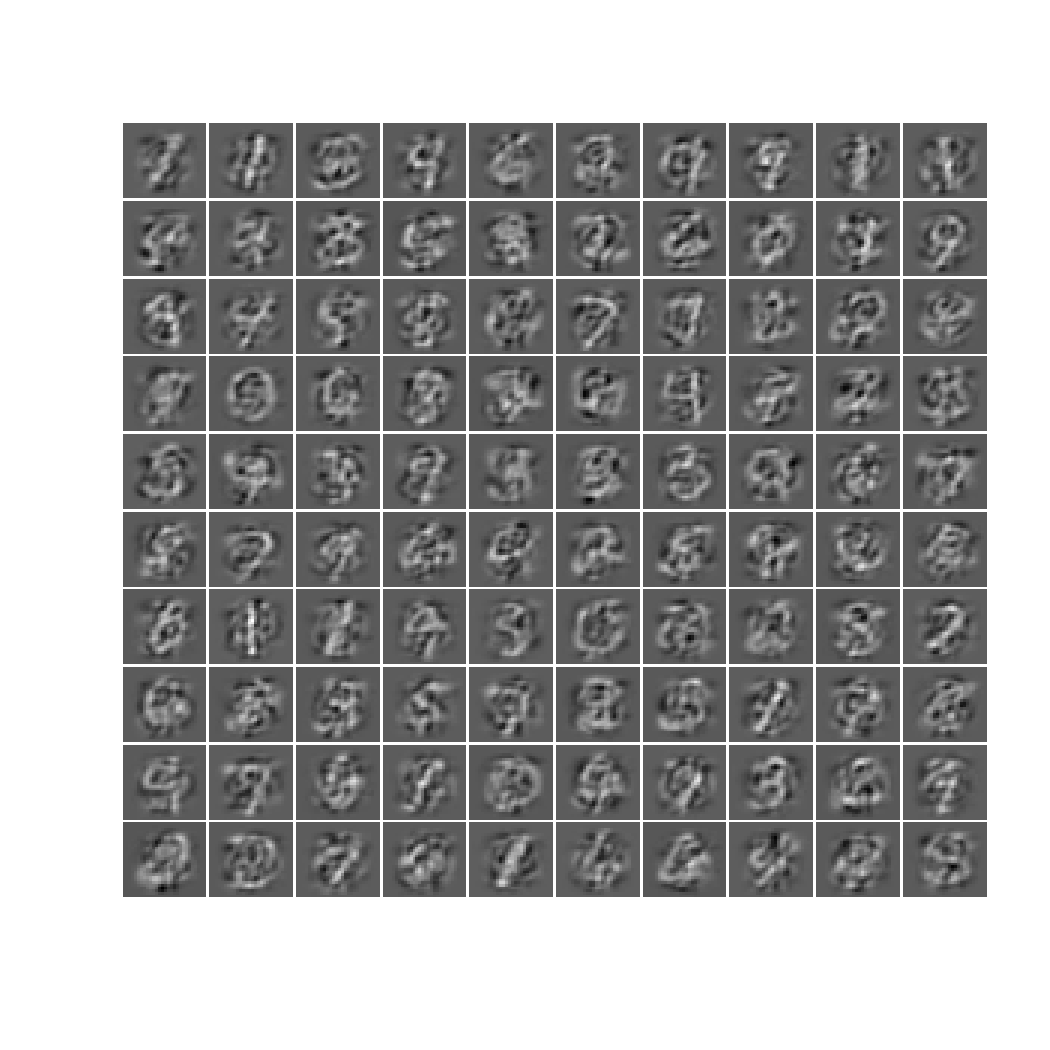
\includegraphics[scale=\dns]{denoise64}
	\caption{}\label{fig:denoise}
\end{figure}

\end{document}
